%!TEX program = xelatex+makeindex+bibtex
\documentclass[final]{scrreprt} %scrreprt of scrartcl
% Include all project wide packages here.
\usepackage{fullpage}
\usepackage{polyglossia}
\setmainlanguage{english}
\usepackage{csquotes}
\usepackage{graphicx}
\usepackage{epstopdf}
\usepackage{pdfpages}
\usepackage{caption}
\usepackage[list=true]{subcaption}
\usepackage{float}
\usepackage{standalone}
\usepackage{import}
\usepackage{tocloft}
\usepackage{wrapfig}
\usepackage{authblk}
\usepackage{array}
\usepackage{booktabs}
\usepackage[toc,page,title,titletoc]{appendix}
\usepackage{xunicode}
\usepackage{fontspec}
\usepackage{pgfplots}
\usepackage{SIunits}
\usepackage{units}
\pgfplotsset{compat=newest}
\pgfplotsset{plot coordinates/math parser=false}
\newlength\figureheight 
\newlength\figurewidth
\usepackage{amsmath}
\usepackage{mathtools}
\usepackage{unicode-math}
\usepackage[
    backend=bibtexu,
	texencoding=utf8,
bibencoding=utf8,
    style=ieee,
    sortlocale=en_US,
    language=auto
]{biblatex}
\usepackage{listings}
\newcommand{\includecode}[3][c]{\lstinputlisting[caption=#2, escapechar=, style=#1]{#3}}
\newcommand{\superscript}[1]{\ensuremath{^{\textrm{#1}}}}
\newcommand{\subscript}[1]{\ensuremath{_{\textrm{#1}}}}


\newcommand{\chapternumber}{\thechapter}
\renewcommand{\appendixname}{Bijlage}
\renewcommand{\appendixtocname}{Bijlagen}
\renewcommand{\appendixpagename}{Bijlagen}

\usepackage[hidelinks]{hyperref} %<--------ALTIJD ALS LAATSTE

\renewcommand{\familydefault}{\sfdefault}

\setmainfont[Ligatures=TeX]{Myriad Pro}
\setmathfont{Asana Math}
\setmonofont{Lucida Console}

\usepackage{titlesec, blindtext, color}
\definecolor{gray75}{gray}{0.75}
\newcommand{\hsp}{\hspace{20pt}}
\titleformat{\chapter}[hang]{\Huge\bfseries}{\chapternumber\hsp\textcolor{gray75}{|}\hsp}{0pt}{\Huge\bfseries}
\renewcommand{\familydefault}{\sfdefault}
\renewcommand{\arraystretch}{1.2}
\setlength\parindent{0pt}

%For code listings
\definecolor{black}{rgb}{0,0,0}
\definecolor{browntags}{rgb}{0.65,0.1,0.1}
\definecolor{bluestrings}{rgb}{0,0,1}
\definecolor{graycomments}{rgb}{0.4,0.4,0.4}
\definecolor{redkeywords}{rgb}{1,0,0}
\definecolor{bluekeywords}{rgb}{0.13,0.13,0.8}
\definecolor{greencomments}{rgb}{0,0.5,0}
\definecolor{redstrings}{rgb}{0.9,0,0}
\definecolor{purpleidentifiers}{rgb}{0.01,0,0.01}


\lstdefinestyle{csharp}{
language=[Sharp]C,
showspaces=false,
showtabs=false,
breaklines=true,
showstringspaces=false,
breakatwhitespace=true,
escapeinside={(*@}{@*)},
columns=fullflexible,
commentstyle=\color{greencomments},
keywordstyle=\color{bluekeywords}\bfseries,
stringstyle=\color{redstrings},
identifierstyle=\color{purpleidentifiers},
basicstyle=\ttfamily\small}

\lstdefinestyle{c}{
language=C,
showspaces=false,
showtabs=false,
breaklines=true,
showstringspaces=false,
breakatwhitespace=true,
escapeinside={(*@}{@*)},
columns=fullflexible,
commentstyle=\color{greencomments},
keywordstyle=\color{bluekeywords}\bfseries,
stringstyle=\color{redstrings},
identifierstyle=\color{purpleidentifiers},
}

\lstdefinestyle{matlab}{
language=Matlab,
showspaces=false,
showtabs=false,
breaklines=true,
showstringspaces=false,
breakatwhitespace=true,
escapeinside={(*@}{@*)},
columns=fullflexible,
commentstyle=\color{greencomments},
keywordstyle=\color{bluekeywords}\bfseries,
stringstyle=\color{redstrings},
identifierstyle=\color{purpleidentifiers}
}

\lstdefinestyle{vhdl}{
language=VHDL,
showspaces=false,
showtabs=false,
breaklines=true,
showstringspaces=false,
breakatwhitespace=true,
escapeinside={(*@}{@*)},
columns=fullflexible,
commentstyle=\color{greencomments},
keywordstyle=\color{bluekeywords}\bfseries,
stringstyle=\color{redstrings},
identifierstyle=\color{purpleidentifiers}
}

\lstdefinestyle{xaml}{
language=XML,
showspaces=false,
showtabs=false,
breaklines=true,
showstringspaces=false,
breakatwhitespace=true,
escapeinside={(*@}{@*)},
columns=fullflexible,
commentstyle=\color{greencomments},
keywordstyle=\color{redkeywords},
stringstyle=\color{bluestrings},
tagstyle=\color{browntags},
morestring=[b]",
  morecomment=[s]{<?}{?>},
  morekeywords={xmlns,version,typex:AsyncRecords,x:Arguments,x:Boolean,x:Byte,x:Char,x:Class,x:ClassAttributes,x:ClassModifier,x:Code,x:ConnectionId,x:Decimal,x:Double,x:FactoryMethod,x:FieldModifier,x:Int16,x:Int32,x:Int64,x:Key,x:Members,x:Name,x:Object,x:Property,x:Shared,x:Single,x:String,x:Subclass,x:SynchronousMode,x:TimeSpan,x:TypeArguments,x:Uid,x:Uri,x:XData,Grid.Column,Grid.ColumnSpan,Click,ClipToBounds,Content,DropDownOpened,FontSize,Foreground,Header,Height,HorizontalAlignment,HorizontalContentAlignment,IsCancel,IsDefault,IsEnabled,IsSelected,Margin,MinHeight,MinWidth,Padding,SnapsToDevicePixels,Target,TextWrapping,Title,VerticalAlignment,VerticalContentAlignment,Width,WindowStartupLocation,Binding,Mode,OneWay,xmlns:x}
}

%defaults
\lstset{
basicstyle=\ttfamily\small,
extendedchars=false,
numbers=left,
numberstyle=\ttfamily\tiny,
stepnumber=1,
tabsize=4,
numbersep=5pt
}
\addbibresource{../../library/bibliography.bib}
\documentclass{article}
\usepackage{listings}
\usepackage{color} %red, green, blue, yellow, cyan, magenta, black, white
\definecolor{mygreen}{RGB}{28,172,0} % color values Red, Green, Blue
\definecolor{mylilas}{RGB}{170,55,241}

\begin{document}


\lstset{language=Matlab,%
    %basicstyle=\color{red},
    breaklines=true,%
    morekeywords={matlab2tikz},
    keywordstyle=\color{blue},%
    morekeywords=[2]{1}, keywordstyle=[2]{\color{black}},
    identifierstyle=\color{black},%
    stringstyle=\color{mylilas},
    commentstyle=\color{mygreen},%
    showstringspaces=false,%without this there will be a symbol in the places where there is a space
    numbers=left,%
    numberstyle={\tiny \color{black}},% size of the numbers
    numbersep=9pt, % this defines how far the numbers are from the text
    emph=[1]{for,end,break},emphstyle=[1]\color{red}, %some words to emphasise
    %emph=[2]{word1,word2}, emphstyle=[2]{style},    
}


\chapter{Assignment 1}
\label{ch:sk5-ass1-task1}
\section{Task 1}
\begin{center}
$Z_s = \dfrac{1}{j \omega C}$\,\,\,\, $Z_p = j \omega L$

$Z_0 = \dfrac{Z_s}{2} + \sqrt{\dfrac{(Z_s)^2}{4} + Z_s \cdot Z_p}$

$Z_0 = \dfrac{1}{2j \omega C} + \sqrt{\dfrac{(\dfrac{1}{j \omega C})^2}{4} + \dfrac{1}{j \omega C} \cdot j \omega L}$

\begin{equation}
Z_0 = \dfrac{1}{2j \omega C} + \sqrt{\dfrac{L}{C} - \dfrac{1}{\omega^2 C^2 4}}
\end{equation}
\end{center}
For $\lim{\Delta  L\to 0}$ the values of the series capacitance $\Delta C$ and shunt inductance $\Delta L$ decrease. The ratio $\Delta L$ and $\Delta C$ will remain constant while the fractions beneath and infront of the square root will approach zero. 
This results in the characteristic impedance:
\begin{equation}
Z_0 = \sqrt{\dfrac{\Delta L}{\Delta C}}
\end{equation}
The cutoff frequency is:
\begin{equation}
W_0 = \sqrt{\dfrac{1}{4LC}}
\end{equation}\\
\\
To determine how the network behaves filter-wise we use the following equation: $V_n = \gamma^n U$. 
This equation gives the voltage at the n-th section of the ladder network.\\
The factor $\gamma$ is equal to $1 - \dfrac{Z_s}{Z_0}$.
With $Z_s = \dfrac{1}{j \omega c}$ we work out the equation to end up at:
\begin{align}
\gamma = \dfrac{\sqrt{\dfrac{L}{C} - \dfrac{1}{\omega^2 C^2 4}} - \dfrac{1}{2j \omega C}}{\sqrt{\dfrac{L}{C} - \dfrac{1}{\omega^2 C^2 4}} + \dfrac{1}{2j \omega C}}
\end{align}
\\For $\lim{\omega \to \infty}$ $\gamma$ approaches 1 and thus the network behaves as a high-pass filter.

\label{ch:sk5-ass1-task2}
\section{Task 2}
The space-time domain of the voltage across the channel equals:
\begin{align}
\label{eq:space-time}
V(z,t) = U(t-\gamma z) + \Gamma U(t + \gamma(z-2l)) - \Gamma U(t-\gamma(z+2l)) - \Gamma^2U(t+\gamma(z-4l))....
\end{align}
With $\Gamma = \dfrac{Z_l - Z_0}{Z_l + Z_0}$ and $z = l$. 
In case the terminal is open there will be an infinite load impedance i.e. $Z_l = \infty$. 
As a consequence $\Gamma = 1$. 
Thus resulting in the following space-time expression 
\begin{align*}
V(z,t) = U(t-\gamma l) + U(t + \gamma(-l)) - U(t-\gamma(3l)) - U(t+\gamma(-3l))....
\end{align*}
Similarly, if the terminal is short-circuited $Z_l = 0$ and $\Gamma = -1$. 
Resulting in the following space-time expression:
\begin{align*}
V(z,t) = U(t-\gamma l) + -U(t + \gamma(-l)) + U(t-\gamma(3l)) - U(t+\gamma(-3l))....
\end{align*}

A positive reflection coefficient points to a positively reflected wave while a negative reflection coefficient points to a negatively reflected wave.

\label{ch:sk5-ass1-task3}
\section{Task 3}
To gain insight in the behavior of the voltage and current in a transmission line a space-time evolution is set up.
The transmission line has the following parameters: 
\begin{itemize}
\item $L_0 = 0.5$ $\mu$H
\item $C_0 = 2$ pF
\item $Z_l = 100$ $\Omega$
\end{itemize}

Accordingly the charactersistic impedance is equal to:
\begin{equation}
Z_0 = \sqrt{\dfrac{L_0}{C_0}} = 500 \Omega
\end{equation}

The transmission line is excited by a rectangular pulse with the following expression:
\begin{equation}
\label{eq:rectangularpulse}
U(t) = V_{max} \cdot \{\epsilon(t) - \epsilon(t-t_w)\}
\end{equation}

In equation \ref{eq:rectangularpulse} $U(t)$ stand for the feeding voltage pulse, $V_{max}$ for the pulse amplitude, $t_w$ for the pulse width and $\epsilon(t)$ for the Heaviside unit step function. 
For the space-time evolution of the voltage equation \ref{eq:space-time} is implemented in MatLab. 
For the space-time evolution of the current we had to re-write some formules to get to an eqution of the form I(z,t). 
The differential equation of the current can be written as: 
\begin{equation} \label{eq:partial}
\frac{\partial^2I(z,t)}{\partial z^2}=C_{0}L_{0}\frac{\partial I(z,t)}{\partial t^2}
\end{equation}
The Laplace transformed of equation \ref{eq:partial} gives us:
\begin{equation} \label{eq:laplace}
\frac{\partial^2\hat{I}(z,s)}{\partial z^2} - C_{0}L_{0}s^2\hat{I}(z,s)=0
\end{equation}
Equation \ref{eq:laplace} in the Laplace domain is a differential equation and heas the following solution: 
\begin{equation} \label{eq:algemeen}
\hat{I}(z,s)=\hat{I}^{+}_{0}(s)e^{-s\gamma z} + \hat{I}^{-}_{0}(s)e^{s\gamma z}
\end{equation}
In equation \label{eq:algemeenI} the coefficients $\hat{I}^{+}_{0}$ and $\hat{I}^{-}_{0}$ can be written as:
\begin{equation} \label{eq:iplus}
\hat{I}^{+}_{0}= \frac{\hat{V}^{+}_{0}(s)}{Z_{0}}
\end{equation}
\begin{equation} \label{eq:imin}
\hat{I}^{-}_{0}= \frac{-\hat{V}^{-}_{0}(s)}{Z_{0}}
\end{equation}
The coefficients $\hat{V}^{+}_{0}$ and $\hat{V}^{-}_{0}$ in equation \ref{eq:iplus} and \ref{eq:imin} can also be written as:
\begin{equation} \label{eq:vplus}
\hat{V}^{+}_{0}= \frac{U(s)}{1 + \hat{\Gamma}(s)e^{-2s\gamma l}}
\end{equation}
\begin{equation} \label{eq:vmin}
\hat{V}^{-}_{0}= \frac{U(s)\hat{\Gamma}(s)e^{-2s\gamma l}}{1 + \hat{\Gamma}(s)e^{-2s\gamma l}}
\end{equation}
By filling in the voltages in equation \ref{eq:vplus} and \ref{eq:vmin} in the equations of the currents in equations \ref{eq:iplus} en \ref{eq:imin}, and in the end putting it al back into the differential equation of the current in equation \ref{eq:algemeenI} we achieve the following:
\begin{equation} \label{eq:volledigI}
\hat{I}(z,s)=\frac{U(s)}{Z_{0}}\left(\frac{e^{-s\gamma z} - \hat{\Gamma}(s)e^{s\gamma (-2l+z)}}{1 + \hat{\Gamma}(s)e^{-2s\gamma l}}\right)
\end{equation}
The geometric series representation of equation \ref{eq:volledigI} is shown below:
\begin{equation} \label{eq:geom}
\hat{I}(z,s)= \frac{U(s)}{Z_{0}}\left(e^{-s\gamma z} - \hat{\Gamma}(s)e^{s\gamma(-2l+z)}\right)\left(1-\Gamma e^{-2s\gamma l}+\Gamma^2 e^{-4s\gamma l}...\right)
\end{equation}
By taking the inverse Laplace transform of equation \ref{eq:geom} we get the following space-time expression for the current:
\begin{equation}
I(t,z)=\frac{u(t-\gamma z)}{Z_{0}}-\frac{\Gamma}{Z_{0}}u(t+\gamma(-2l+z))-\frac{\Gamma}{Z_{0}}u(t+\gamma(-2l-z)) + \frac{\Gamma^2}{Z_{0}}u(t+\gamma(-4l+z))
\end{equation}
\\
Consequently the space-time evolution can be plotted with help of the given function \texttt{Bscan\_plot.m}. For equation \ref{eq:rectangularpulse} we made a new function, \texttt{U.m}. This function can be seen below. \\
\lstinputlisting{Matlab/U.m}
\\
Before we could write the Matlab code we first had to define the following parameters:
\begin{itemize}
\item $V_{max}$ = 1 V
\item $t_w$ = 0.5 ns
\item t $\in$ [0.5] ns
\item x $\in$ [0,1.2] m
\end{itemize}

The written Matlab code for plotting the space-time evolution of the current I(x,t) and voltage V(x,t) can be seen below. 
\lstinputlisting{Matlab/task3.m}

\begin{figure}[H]
	\centering
	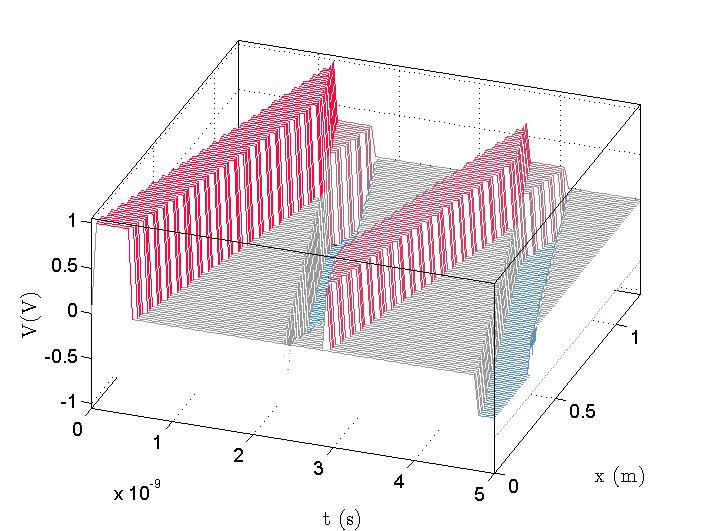
\includegraphics[width=\linewidth]{resources/task3.png}
	\caption{Space time evolution of the voltage.}
	\label{fig:space-time-voltage}
\end{figure}
As can be seen in figure \ref{fig:space-time-voltage} the signal propagates through the transmission channel and reflects negatively because the reflection coefficient is a negative number. Because this coefficient is bigger than -1 the reflected signal decreases in amplitude.

The plot of the space-time evolution of the current $I(z,t)$ can be seen in figure \ref{fig:iplot}. 
\begin{figure}[H]
\centering
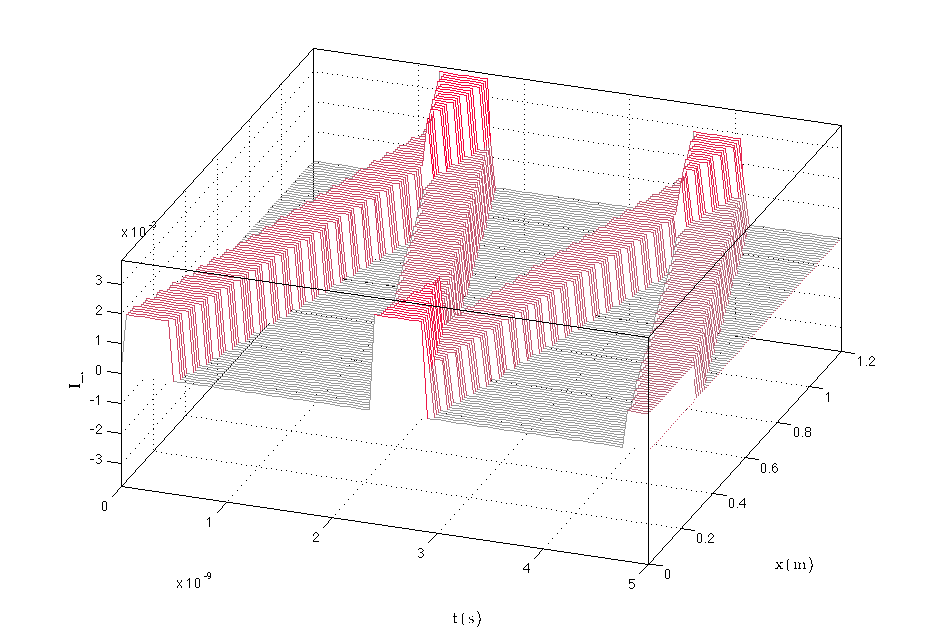
\includegraphics[width=\linewidth]{resources/Iplot.png}
\caption{Space time evolution of the current.}
\label{fig:iplot}
\end{figure}

\



\end{document}